% Chapter 3

\chapter{Study of Wu et. al.'s algorithm for locally optimal NAMO in unknown environments} % Main chapter title

\label{Chapter3} % For referencing the chapter elsewhere, use \ref{Chapter3}

\paragraph{} Given the state of the art presented in the previous chapter and what we aimed to achieve in the available time, we chose to build upon Wu et. al.'s algorithm for locally optimal NAMO in unknown environments.

\section{Original algorithms}

\paragraph{} In Wu et. al.'s proposition, the basic idea is to consider either a plan that doesn't involve interacting with obstacles (which can be achieved with any pre-existing path finding algorithm), or a three-steps plan that consists in, first, reaching the obstacle ($c_{1}$), second, pushing it in a single direction ($c_{2}$), and finally reaching the goal from the position we left the obstacle at ($c_{3}$). This is best shown in figure \ref{fig:Wu_Original_Algorithm-wu_components_illus}.

\begin{figure}[H]
\centering
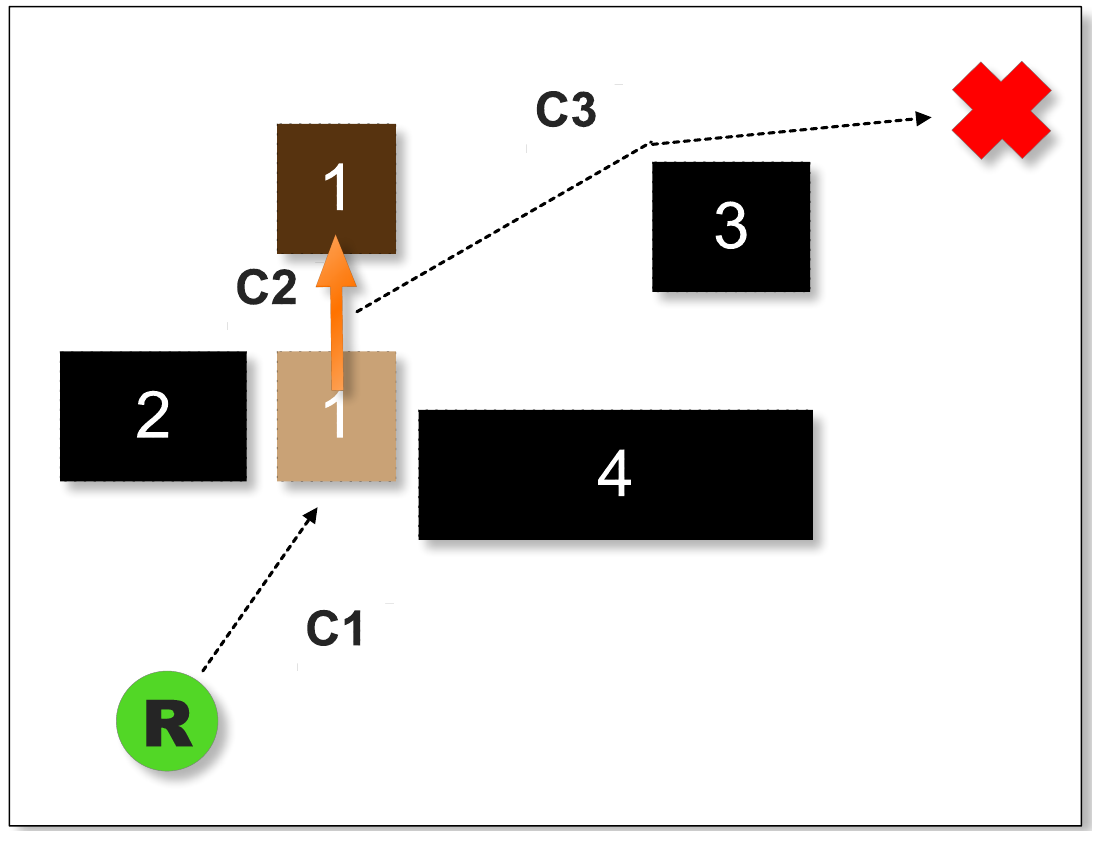
\includegraphics[width=5cm]{Figures/Wu_Original_Algorithm/wu_components_illus.png}
\caption{Figure describing the three plan components when pushing an object, as published in \parencite{wu_navigation_2010}.}
\label{fig:Wu_Original_Algorithm-wu_components_illus}
\end{figure}

\paragraph{} In their first article \parencite{wu_navigation_2010}, Wu et. al. describe two versions of their algorithm: a naive but locally optimal baseline one, and an optimized one, built upon the logic foundation of the first, but that loses its local optimality. In their second article \parencite{levihn_locally_2014}, several other improvements on performance are proposed that restore the local optimality of the proposition. By locally optimal, we mean that the algorithm will \textbf{always} choose the \textbf{best} plan given its current, limited knowledge of the environment.

\paragraph{} The baseline algorithm is very straightforward: it uses an A* path finding subroutine to determine the optimal path between the current robot's position and the goal, avoiding all known obstacles (none at the beginning). As the robot moves forward (Figure \ref{fig:Wu_Original_Algorithm-algo1}, line 17), and therefore gains new information (same figure, line 5), whenever a new obstacle is encountered, every push action for every obstacle is re-simulated (Figure \ref{fig:Wu_Original_Algorithm-algo2}) and compared to the current optimal plan (Figure \ref{fig:Wu_Original_Algorithm-algo1}, line 11). Local optimality is guaranteed for this approach, since the A* algorithm is used with the admissible Euclidean heuristic, thus returning optimal solutions for a given state of the map and goal, and also because whenever a new obstacle is detected (= the map is in a new state), \textbf{all} possible plans are re-evaluated and compared to check if a better plan than the current one can be found or not before moving the robot again.

\begin{figure}[H]
\centering
\begin{subfigure}{.5\textwidth}
  \centering
  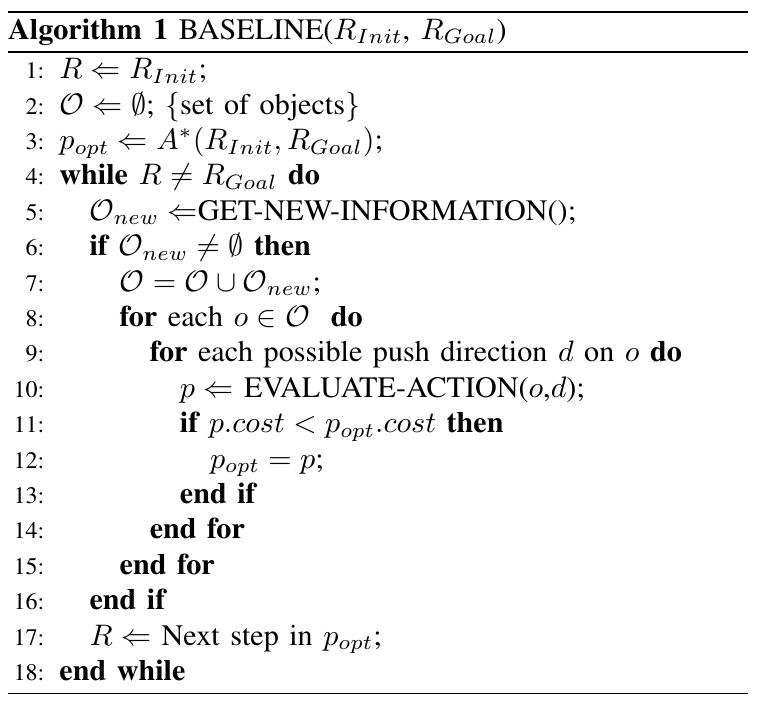
\includegraphics[width=\linewidth]{Figures/Wu_Original_Algorithm/algo1.png}
  \caption{Main loop that evaluates all plans containing the manipulation of an obstacle every time a new one is found}
  \label{fig:Wu_Original_Algorithm-algo1}
\end{subfigure}%
\begin{subfigure}{.5\textwidth}
  \centering
  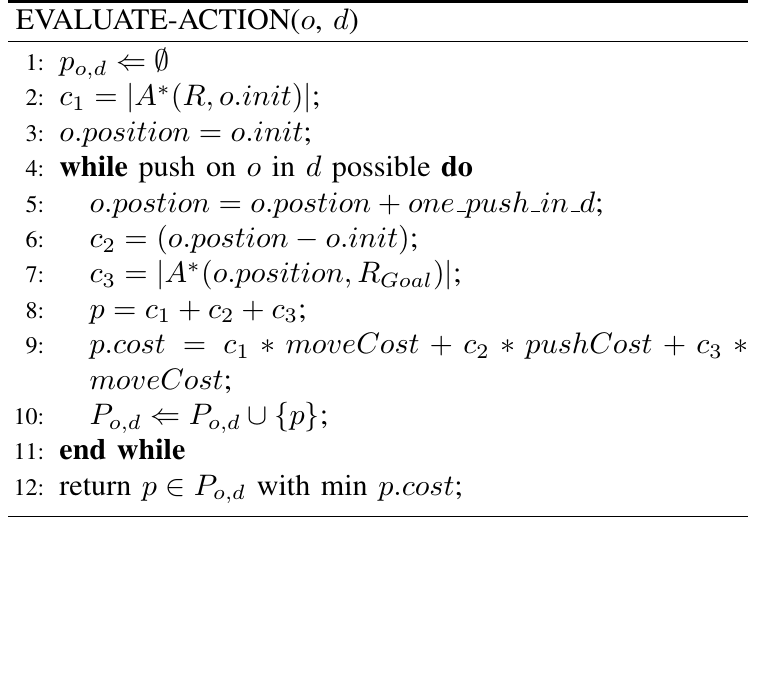
\includegraphics[width=\linewidth]{Figures/Wu_Original_Algorithm/algo2.png}
  \caption{Subroutine for evaluating all possible plans for each manipulation direction allowed on an obstacle}
  \label{fig:Wu_Original_Algorithm-algo2}
\end{subfigure}
\caption{Baseline Algorithm as published by Wu et. al. in \parencite{wu_navigation_2010}}
\label{fig:Wu_Original_Algorithm-baseline}
\end{figure}

\paragraph{} The optimized version of the algorithm published in the first article offers four optimization steps:

\paragraph{First Optimization}\label{optimization_1} Only consider computing a new plan if the current one is actually blocked by a new obstacle (Figure \ref{fig:Wu_Original_Algorithm-algo3}, line 6). This keeps the local optimality, since a newly detected obstacle can only imply a costlier plan either moving around it or moving it (\textbf{assuming obstacles don't move by themselves, which could open new, better routes}): given that we can assume that our current optimal plan was optimal before the discovery of the new obstacle, we need only reconsider it if the new obstacle actually prevents it from coming to fruition.

\paragraph{Second Optimization}\label{optimization_2} Stop simulating pushes in a given direction before it becomes costlier than the current valid optimal plan, thanks to a bound (Figure \ref{fig:Wu_Original_Algorithm-algo4}, line 5). This also keeps optimality, since there are no reasons to continue evaluating actions that are already costlier than simply following the current valid optimal plan.

\paragraph{Third Optimization}\label{optimization_3} Only compute the third path component (from obstacle to goal) with A* if the simulated movement actually creates an opening (Figure \ref{fig:Wu_Original_Algorithm-algo4}, line 7), since checking an opening creation is less computing time-consuming than running a search algorithm to the goal. However, this step also causes the loss of local optimality, because it prevents the algorithm to fully evaluate some plans that could improve the cost. Below are examples figures of cases where this happens, assuming the cost of following a path is the same whether it implies moving an obstacle or not. In Figure \ref{fig:corridor_case} and \ref{fig:openspace_case}, no new opening is ever found, either because the blocking areas around the obstacle don't change (\ref{fig:corridor_case}) or because there were no blocking areas to begin with (\ref{fig:openspace_case}). Theses case are tentatively adressed in Chapter \ref{Chapter4}.

\begin{figure}[H]
\centering
\begin{subfigure}{.5\textwidth}
  \centering
  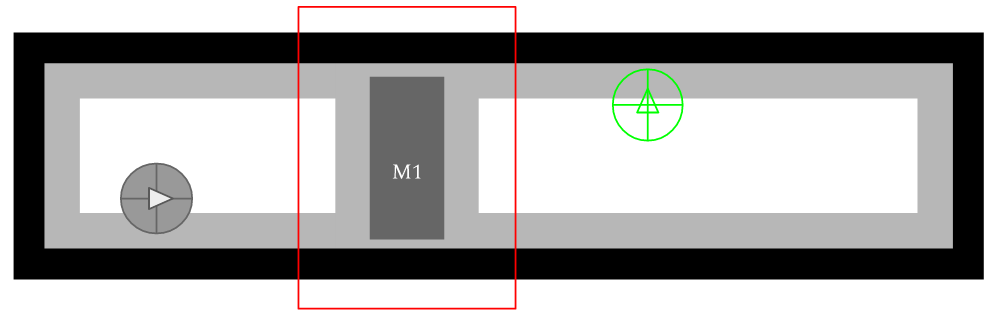
\includegraphics[width=\linewidth]{Figures/Check_New_Opening/corridor_original.png}
  \caption{Initial situation.}
  \label{fig:corridor_original}
\end{subfigure}%
\begin{subfigure}{.5\textwidth}
  \centering
  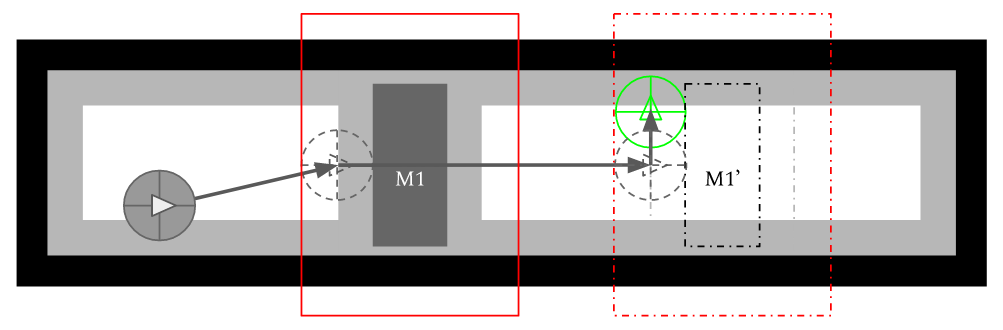
\includegraphics[width=\linewidth]{Figures/Check_New_Opening/corridor_optimal_path.png}
  \caption{Expected plan.}
  \label{fig:corridor_optimal_path}
\end{subfigure}
\caption{"Corridor" case where the original algorithm will not even find a plan when it should.}
\label{fig:corridor_case}
\end{figure}

\begin{figure}[H]
\centering
\begin{subfigure}{.45\textwidth}
  \centering
  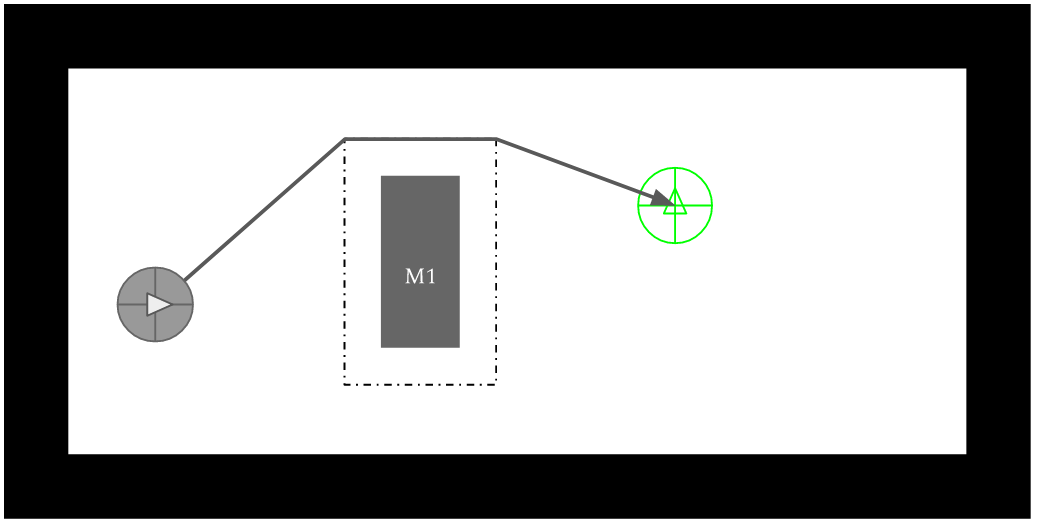
\includegraphics[width=\linewidth]{Figures/Check_New_Opening/openspace_original.png}
  \caption{Initial situation and suboptimal plan avoiding the obstacle that will be returned by the original algorithm.}
  \label{fig:openspace_original}
\end{subfigure}%
\begin{subfigure}{.45\textwidth}
  \centering
  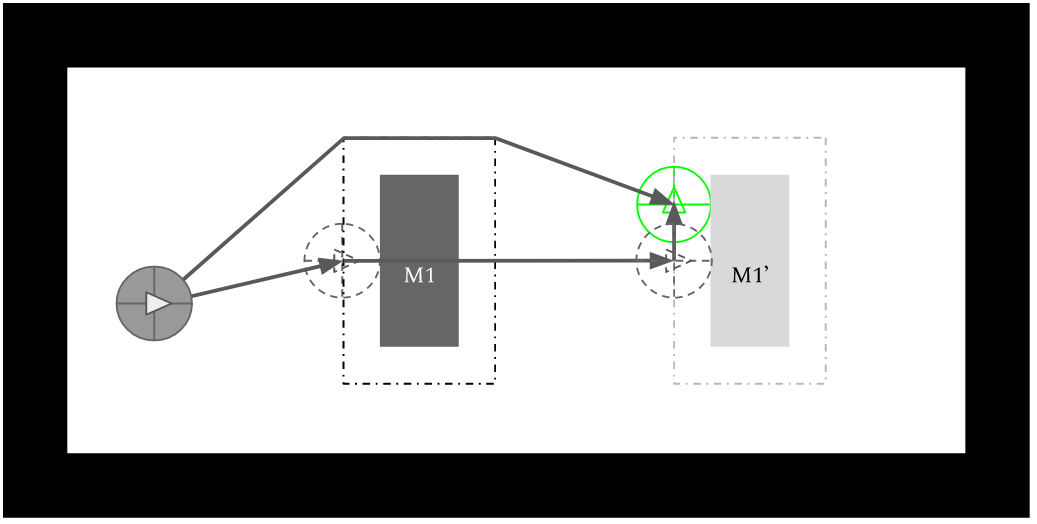
\includegraphics[width=\linewidth]{Figures/Check_New_Opening/openspace_optimal_path.png}
  \caption{Expected plan is the one that pushes the obstacle.}
  \label{fig:openspace_optimal_path}
\end{subfigure}
\caption{"Open space" case where the original algorithm will find only a suboptimal plan.}
\label{fig:openspace_case}
\end{figure}

\paragraph{Fourth Optimization}\label{optimization_4} Finally, when the plan needs to be re-evaluated, new obstacles are evaluated first(Figure \ref{fig:Wu_Original_Algorithm-algo3}, lines 8 to 12) and the resulting paths are saved into a list (Figure \ref{fig:Wu_Original_Algorithm-algo3}, lines 2 and 10) by growing order of an underestimated heuristic cost that corresponds to sum of the costs of the plan components $c_{2}$ and $c_{3}$ (Figure \ref{fig:Wu_Original_Algorithm-algo4}, line 12). Then, this list is used to iterate over all obstacle/push direction combinations, and re-evaluate the corresponding plan (Figure \ref{fig:Wu_Original_Algorithm-algo3}, lines 13 to 20). The re-evaluation can be stopped as soon as the next pair to consider has a heuristic cost greater than the cost of the current optimal plan, improving execution performance (Figure \ref{fig:Wu_Original_Algorithm-algo4}, line 14). However, this optimization step causes the loss of the guarantee of optimality. The heuristic cost depends on $c_{2}$ and $c_{3}$, and when moving an obstacle, these components' costs may get lower. As the algorithm never updates the heuristic cost ($minCost$) in the list according to this possibility, there is therefore no guarantee that the heuristic cost will always be an underestimate. In the words of Levihn, main author of the second article:  \textit{"Second, as the algorithm does not acknowledge the fact that free-space can be created during the execution (e.g. by moving objects), which can lower c2 or c3 for some objects, this optimization steps sacrifices local optimality."} \parencite{levihn_locally_2014}

\paragraph{Note on the use of A* in the main loop} In Figure \ref{fig:Wu_Original_Algorithm-algo3}, lines 3 and 7, a call to the A* algorithm is made. For line 3, it determines the optimal path from the initial position to the goal, supposing no obstacle has been detected yet. In line 7, after the current optimal path has been invalidated by the detection of a collision between this path and a new obstacle, this call to A* star allows to get a new optimal path that avoids all obstacles that will serve as basis for the comparison with paths that consider moving obstacles.

\begin{figure}[H]
\centering
\begin{subfigure}{.45\textwidth}
  \centering
  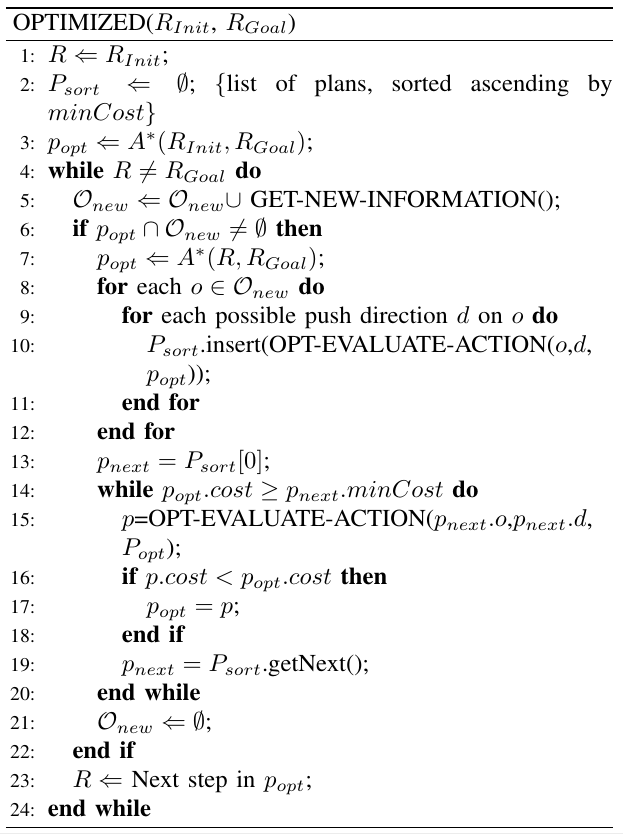
\includegraphics[width=\linewidth]{Figures/Wu_Original_Algorithm/algo3.png}
  \caption{Main loop}
  \label{fig:Wu_Original_Algorithm-algo3}
\end{subfigure}%
\begin{subfigure}{.45\textwidth}
  \centering
  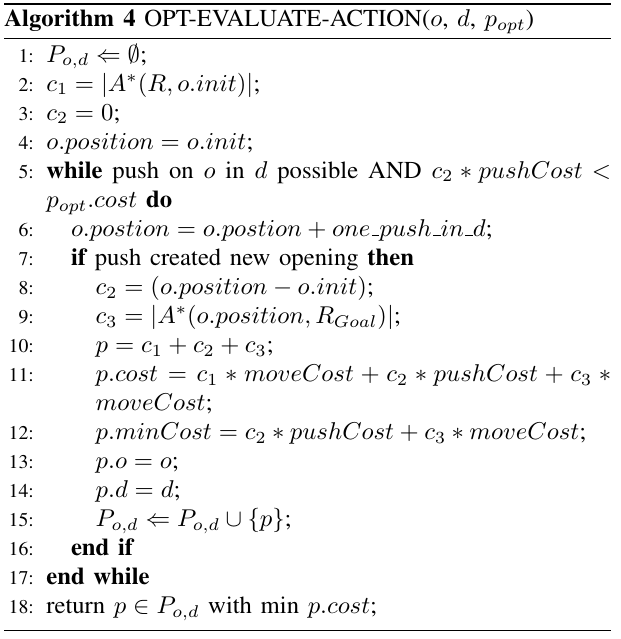
\includegraphics[width=\linewidth]{Figures/Wu_Original_Algorithm/algo4.png}
  \caption{Subroutine}
  \label{fig:Wu_Original_Algorithm-algo4}
\end{subfigure}
\caption{Optimized Algorithm as published by Wu et. al. in \parencite{wu_navigation_2010}}
\label{fig:Wu_Original_Algorithm-optimized}
\end{figure}

\section{Removing ambiguity}\label{removing_ambiguity_section}
\paragraph{} The original pseudocode presented above has quite a few typos, implicit or incongruous notations that create ambiguity (e.g., storing costs and paths in the same variable, having two different variable affectation operators ($\gets$ and $=$), ...), confusing the reading. Since no pseudocode is provided by the authors for the second article's improvements propositions, it was necessary to first fix the pseudocode of the first article. The following paragraphs and the pseudocode formulation \ref{appendix_reworked_wu_section} in Appendix \ref{algorithms} aim at fixing this.

\paragraph{A foreword on notations:}

\begin{itemize}
  \item Paths are ordered sets of "steps", which are themselves robot poses.
  \item Calling the A* or D*Lite algorithms returns A PATH. If no path is found, the returned set is empty: $\emptyset$.
  \item Plans are to be noted with a lowercase $p$. Lists or sets of plans will be noted with an uppercase $P$. A plan is a data structure with a "components" list attribute in which paths are stored in order of execution, and a "cost" attribute that represents the cost of executing the plan.
  \item Components of a plan are noted with a lowercase $c$.
  \item Assuming we suppose a cost in distance, the norm of a path $path$ (written $|path|$) corresponds to the sum of the euclidean distances between consecutive steps, and $+\infty$ if the path is empty.
  \item $moveCost$ and $pushCost$ are constants without dimension.
  \item The current robot pose is to be noted with an uppercase $R$, the initial pose with $R_{init}$ and the goal pose with $R_{goal}$
  \item Obstacles are to be noted with a lowercase $o$. Lists or sets of obstacles will be noted with an uppercase $O$.
\end{itemize}

\paragraph{Note on update}\label{update-from-new-information_note} In the original paper, it is not explicit how the GET-NEW-INFORMATION method works. We therefore changed it to UPDATE-FROM-NEW-INFORMATION() method, that updates the world representation $I$ given in parameter, with new information about obstacles that is collected in parallel in a different execution thread. By that we mean, if this new information includes modifications to known obstacles, they are updated, and if there are new obstacles, they are added to $I$. We assume that the attribute $I$.occGrid corresponds to the occupation grid with inflated obstacles in the current state, so that the path finding routine may run with it. In the same way, $I$.newObstacles corresponds to the list of newly observed obstacles since the last call of the same method.

\paragraph{Note on intersection detection}\label{intersection_note} The $p_{opt} \bigcap \mathcal{O}_{new} \neq \emptyset$ notation is used here as shorthand for checking that any of the new obstacles do not intersect with the robot's path. In implementation, this could be done for example by checking whether every pose in the path is not comprised in the inflated obstacles representation.

\paragraph{Note on re-evaluation}\label{re-evaluation_note} The way the algorithm is written now, even new obstacles that have just been evaluated might be reevaluated, since they have been inserted into the $P_{sort}$ list right before. Consequently, we should add a condition $p_{next}.o \notin \mathcal{O}_{new}$ around the line \ref{lst:line:suppcondition} of Algorithm \ref{alg:01-wu-optimized-part1} to further optimize the algorithm.

\paragraph{Note on getNext}\label{getnext_note} This is a helper method to traverse a list. It returns null when all elements have been traversed.

\paragraph{Note on stop condition}\label{stop_condition_note} The algorithm's stop condition is not explicit in none of the articles. If no path has been found even after considering all relevant obstacles, then the algorithm must return a success value.

\paragraph{Note on plan following}\label{plan_following_note} In the article, the hypothesis is given that if the robot tries to move an obstacle but does not succeed, this obstacle will never be considered for manipulation again. It is meant to allow the robot to detect unmovable obstacles and to avoid an infinite loop caused by an endless evaluation of a same obstacle that cannot be moved. This hypothesis is translated in pseudocode by replacing the vague "$R \gets$ Next step in $p_{opt}$" statement by checking whether the robot actually checking whether robot succeeded or not the desired movement by comparing the actual pose $R_{real}$ after execution and the one we wished to reach $R_{next}$ , and using the $blockedObsL$ set to remember obstacles that should never be evaluated again.

\paragraph{Note on obstacle push pose}\label{obstacle_pushpose_note} For a given obstacle, the algorithm iterates over every push direction applicable to it, but doesn't iterate over every point from which it could apply said push direction. We must deduce that there is an \textbf{implicit hypothesis that for a given push direction, only one point around the obstacle is a valid manipulation start point}. Therefore, we will assume that $o.init$ corresponds to the pose the robot must get into in order to move obstacle $o$ in direction $d$. From the video\footnote{\url{https://youtu.be/oQZLbJHYrl8}} that presents an implementation of the original algorithm, this pose:

\begin{itemize}
  \item Is orientated in the given direction, toward the side of the obstacle that allows to push in the given direction,
  \item Is situated on precomputed "manipulation points" that are at a robot radius distance from the side; often it seems that this point is in front of the side's middle point,
  \item Among these "manipulation points" it seems the one closest to the current position of the robot is chosen. This is fine since the algorithm seems to operate under the \textbf{implicit hypotheses that the friction between the ground and the obstacle is negligible, and that the robot's width is always smaller than the length of the obstacle's side being pushed}. Thus, if the obstacle is movable and not blocked by surrounding obstacles, it will move in the direction it is being pushed in, whatever the accessible "manipulation point" on the appropriate side may be.
\end{itemize}

\paragraph{Note on $c_{1} \neq \emptyset$}\label{c1_note} This condition is not in the original pseudocode, but is necessary to avoid the limit case where no path from the current robot pose to the obstacle is found, in which case, the manipulation plan cannot exist.

\paragraph{Note on bounding}\label{bound_note} It is not said in the article how the "push on $o$ in $d$ possible" condition is verified, but we can assume that it is checked by verifying at each step that the obstacle's new occupied space doesn't intersect with any other obstacle. The $c_{2} * pushCost$ bound here is not tight at all, which is fixed in the new optimization steps proposed in the second article. Still, it allows to cut down on unnecessary evaluations of extra pushes.

\paragraph{Note on $I.withSimulatedObstacleMove$}\label{i_note} This notation is to explicit the fact that the $c_{3}$ component must be computed assuming that the obstacle has been pushed, otherwise it does not make any sense.

\paragraph{Note on elementary push}\label{push_in_d_note} It is not explicit in the article how an elementary $one\_push\_in\_d$ is computed, but we can assume it is the multiplication of a distance constant by the unit direction vector for the given direction $d$. We will make this more explicit in our own algorithm.

\paragraph{Note on opening detection}\label{opening_detection_note} Opening detection is not adressed in this paper and the method used is not explicit. A technical paper later written by co-authors Levihn and Stilman \parencite{levihn_efficient_2011} however clears this ambiguity: \textit{"The algorithm did not rely on search but simply observed the amount of adjacent free spaces on corners of the manipulated obstacle. While efficient, this algorithm is only applicable for world configurations populated with simple rectangular shaped static and movable obstacles. This is not realistic."}.

\paragraph{Note on $c_{2}$}\label{c2_note} As we only admit pushes in straight lines, and because the previous "push on $o$ in $d$ possible" condition means that there will be no collision on the manipulation path, $c_{2}$ simply is a path made from the pose to start moving the object and the pose where the robot leaves it.

\paragraph{Note on $c_{3} \neq \emptyset$}\label{c3_note} This condition is not in the original pseudocode, but is necessary to avoid the limit case where no path from the obstacle to the goal is found, in which case, the manipulation plan cannot exist.

\section{Pseudocode expression of Levihn's recommendations}

\label{levihn_pseudocode_section}

\paragraph{} In the second article \parencite{levihn_locally_2014}, Levihn brings alternate solutions for the \nameref{optimization_2}, \nameref{optimization_3} and \nameref{optimization_4}, reducing the computational effort and enlarging the scope of problems the algorithm can manage. For the \nameref{optimization_4}, the changes make it so optimality is not affected by this optimization step. Our pseudocode formulation \ref{appendix_levihn_interpretation_section} is available in Appendix \ref{algorithms}.

\paragraph{\nameref{optimization_2}} In this article, the authors precise that they are using an improved opening detection algorithm, detailed in their separate technical paper \parencite{levihn_efficient_2011}. Since contrary to the previous one, this new algorithm doesn't rely on obstacles being rectangles, but accepts any kind of polygon, it extends the capability of the overall algorithm to any convex polygon.

\paragraph{} \textbf{However, in the same way we proved that using opening detection for considering the computation of a full plan affected optimality before, since no measures are proposed in this new article to take this into account, we must assume that local optimality is not restored}. In Chapter \ref{Chapter4}, \hyperref[check_opening_solution]{we propose a measure for restoring optimality}.

\paragraph{\nameref{optimization_3}} The bound that allows to reduce the number of unnecessary evaluations of extra pushes is tightened by adding to the current value of $|c_{2}|$ the cost of the first plan component $c_{1}$ and an underestimate of the cost of the third plan component $c_{3}$. This underestimate is the euclidean distance between the last position of the simulated push pose $oSimPose$ and the goal pose $R_{goal}$. This bound is thus proved to be an underestimate of the real cost, keeping optimality.

\paragraph{\nameref{optimization_4}} Last but not least, a new heuristic is proposed alongside a modified version of the previous one. Basically, all obstacles that haven't been evaluated at least once are ordered in a separate list $euCostL$ by a heuristic cost that is independent from $c_{2}$ and $c_{3}$: the euclidean distance between the goal pose $R_{goal}$ and the obstacle's nearest "manipulation point" at which the robot could manipulate it. When an obstacle has been evaluated, it is added to another list $minCostL$ ordered by the usual $minCost$. Since this heuristic is more informed, $minCostL$ is used first when available. If not, $euCostL$ is used, the obstacle is re-evaluated and naturally added to the list ordered by $minCost$. This is achieved through the use of separate indexes for traversing the lists: $i_{e}$ and $i_{m}$. This heuristic is invalidated anytime an obstacle has changed of place, potentially lowering $c_{2}$ or $c_{3}$. Thus, local optimality is no longer affected. For a more detailed explanation, please consult the following pseudocode or the original article \parencite{levihn_locally_2014}.

\paragraph{Reordering the algorithm} Since this is an interpretation, and for easier understanding, we took the liberty of cutting the "OPTIMIZED" algorithm (main loop) into two algorithms: the main loop where the plan is executed and knowledge about the environment updated (i.e. Algorithm \ref{alg:02-levihn-makeandexecuteplan}: "MAKE-AND-EXECUTE-PLAN"), and the subroutine where the iteration over the obstacles is done to generate a new plan when necessary (i.e Algorithm \ref{alg:02-levihn-makeplan}: "MAKE-PLAN"). We also renamed the "OPT-EVALUATE-ACTION" subroutine (i.e Algorithm \ref{alg:01-wu-optevaluateaction}) into "PLAN-FOR-OBSTACLE" (i.e Algorithm \ref{alg:02-levihn-planforobstacle}). Note that the parameters $p_{opt}$, $euCostL$ and $minCostL$ are directly modified during the execution of the MAKE-PLAN() method, hence no return statement in it.

\paragraph{Note on D*Lite}\label{d_star_note} In the second article, it is mentionned twice that the path finding subroutine has been changed from A* to D*Lite. However, not even a hint of an explanation is given as to why this change, or what difference in the implementation it makes. Therefore, in our later final implementation, we shall stick with A*.

\paragraph{Note on update}\label{second_update-from-new-information_note} In addition to the previous note (\ref{update-from-new-information_note}) We assume that $I$.freeSpaceCreated is True if any obstacle's occupied space has been reduced, False otherwise, and that $I$.allObstacles is the list of all observed obstacles in the current state.

\paragraph{Note on getting the list element and limit cases}\label{get_list_element_note} For the sake of readability in the pseudocode, if the list element that is asked for is out of bounds (empty list or reached end of list), the "[ ]" operator shall return a "fake" tuple with a null obstacle reference, and infinite cost: \{null, $+\infty$\}. This could easily be implented in code by either using a ternary operator (for example, "$minCostL[i_{m}].minCost$" would become "$minCostL[i_{m}] =$ null ? $+\infty: minCostL[i_{m}].minCost$") or implementing a custom array object with the wanted behaviour.

\paragraph{Note on $evaluatedObstacles$}\label{evaluated_obstacles_note} $evaluatedObstacles$ is a set that remembers which obstacles have been evaluated in the current MAKE-PLAN instance. This is not mentioned in the original article, but it avoids evaluating an obstacle twice when it is added to $minCostL$.

\paragraph{Traversal note}\label{list_traversal_note} Stop condition: if the next entry from $minCostL$ or $euCostL$ to be considered (the one with the lowest cost) is associated with a cost that is greater than the current optimal plan, it is not worth trying to evaluate any more options, and therefore the loop must end.

\paragraph{Note on priority}\label{minCostL_priority_note} If the current lowest cost entry is minCostL, evaluate the associated obstacle.

\paragraph{Note on postponing}\label{postponing_note} If $i_{e}$ points to a lower cost than the one pointed by $i_{m}$, we only evaluate the associated object if $minCostL$ doesn't already contain an evaluation for it (because there is tighter bound for the cost of moving the object): the evaluation is thus postponed until the obstacle is reached through $minCostL$.

\paragraph{Note on manipulation points \& $c_{1}$'s computation}\label{c1_computation_note} In the article, the authors claim that \textit{"c1 only needs to be calculated once for the entire process of evaluating the current object."}. With the same reasoning as in \nameref{obstacle_pushpose_note}, this affirmation can only be true if the algorithm operates under the \textbf{implicit hypothesis that for all given manipulation directions, only one point around the obstacle is considered a valid manipulation start point}. From \href{https://youtu.be/3AvfPVzBb-s}{the video} accompanying the article, this point seems to be the nearest point from the robot, situated at a radius distance from the middle of a side of the obstacle. However, this hypothesis actually hinders optimality: if there is in fact a valid manipulation point for each side of the obstacle, and the algorithm knowingly doesn't consider them because they are further from the current robot's position, it will ignore the fact that a same manipulation direction could end up in opening a better path if the obstacle were moved from another manipulation point (see figures below). To guarantee optimality, we would have to simulate the manipulation in the given direction for every reachable manipulation point, thus re-evaluating $c_{1}$ for each. That would result in adding an extra "for" loop englobing the existing one. This is illustrated by the figures below.

\begin{figure}[H]
\centering
\begin{subfigure}{.5\textwidth}
  \centering
  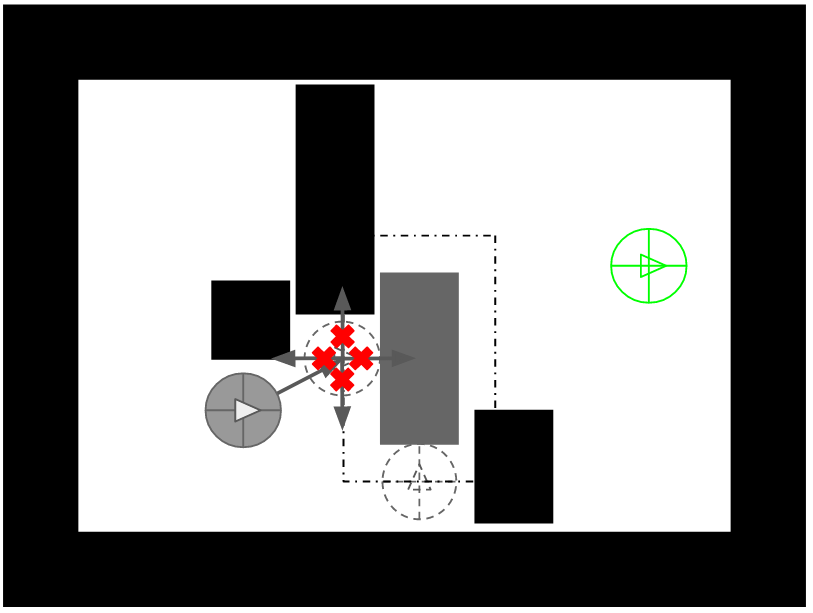
\includegraphics[width=\linewidth]{Figures/Manipulation_Pose/manip_pose_1.png}
  \caption{Nearest manipulation pose doesn't allow moving the obstacle at all.}
  \label{fig:manip_pose_1}
\end{subfigure}%
\begin{subfigure}{.5\textwidth}
  \centering
  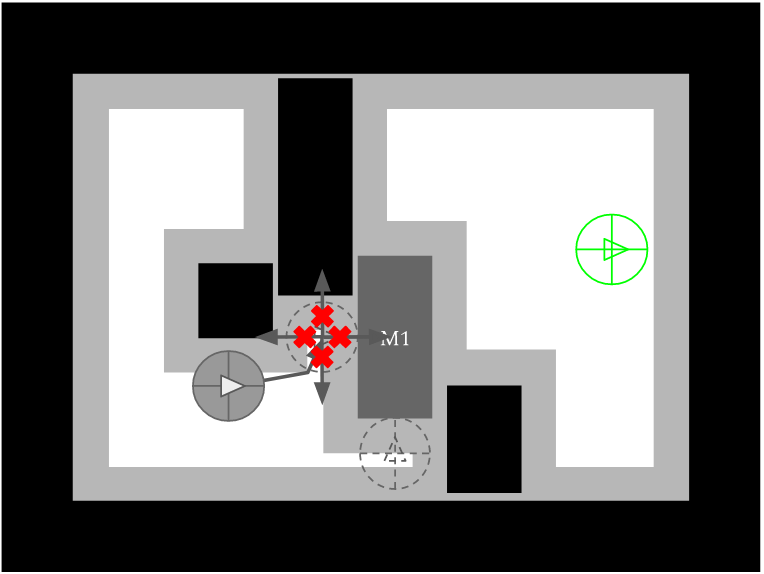
\includegraphics[width=\linewidth]{Figures/Manipulation_Pose/manip_pose_2.png}
  \caption{But if we also consider the other pose, a valid plan can be found.}
  \label{fig:manip_pose_2}
\end{subfigure}
\caption{Illustration of the importance of considering all possibles manipulations for all manipulation poses and not just considering the nearest one.}
\label{fig:manipulation_poses}
\end{figure}

\paragraph{Note on BA}\label{remember_ba_note} The BA variable in the OPT-EVALUATE-ACTION() function allows to remember the initial blocking areas when using the new algorithm for more efficient opening detection. On the first called, the variable is initialized with the initial blocking areas, and at each following call, it is passed as a parameter to reduce computational overhead. This measure is recommended by the technical paper.

\paragraph{Note on allowed manipulations}\label{allowed_manipulations_note} In the second article, the authors assert that they don't limit manipulation to pushes. However, it is clear, especially from \href{https://youtu.be/3AvfPVzBb-s}{the video}, that manipulations are restricted to translations in a single direction.

\paragraph{Note on $seq$}\label{seq_note} Seq corresponds to the number of unit translations that have been simulated.
